% This work is licensed under the Creative Commons
% Attribution-NonCommercial-ShareAlike 4.0 International License. To view a copy
% of this license, visit http://creativecommons.org/licenses/by-nc-sa/4.0/ or
% send a letter to Creative Commons, PO Box 1866, Mountain View, CA 94042, USA.
% vim: set noexpandtab:

\section{Stromlinien-Diffusions-Methode (SDFEM)} %7.
Hughes / Brooks 1979

\subsection{Motivation}
\begin{align*}
\left\lbrace
	\begin{array}{rl}
	-\varepsilon\cdot\Delta u+b\cdot \nabla u+c\cdot u=f&\text{ in }\Omega\\
	u=g&\text{ auf }\Gamma=\partial\Omega\\
	0<\varepsilon\ll 1&
	\end{array}
	\right.
\end{align*}

Für $\varepsilon=0$ ist dies eine PDE erster Ordnung, aber für $\varepsilon>0$ eine PDE zweiter Ordnung.
Beim Grenzübergang passieren "magische Dinge", die sich mit den bisher bekannten Verfahren nicht sinnvoll lösen lassen.
Es kommt zu Oszillationen.
Deshalb wurden die SDFEM-Verfahren erfunden.
Die Idee besteht darin aus das diskrete Problem noch $\delta_K$-mal das glatte Problem dazu zu addieren.\nl
\textbf{1D:}
\begin{align*}
	-\varepsilon\cdot u''+u'=0\text{ auf }(0,1),\qquad u(0)=0,\qquad u(1)=1
\end{align*}
\begin{figure}[!ht]
	\begin{center}
		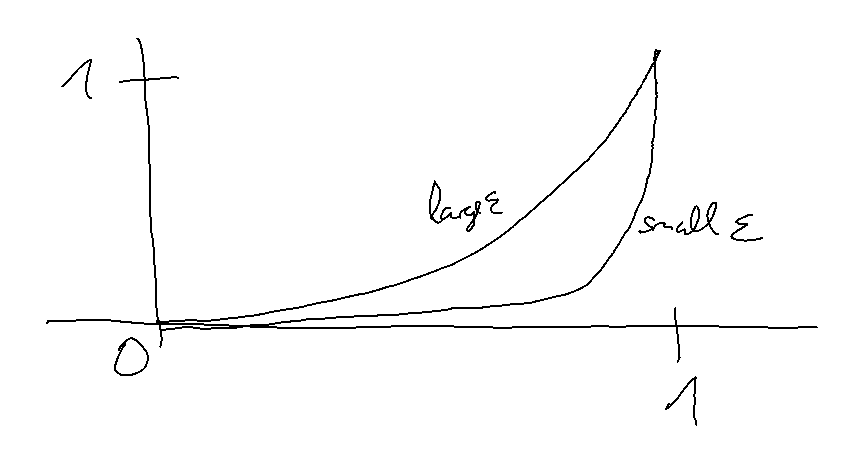
\includegraphics[width=0.7\textwidth]{pics/Sketch16.png}
		\caption{Skizze für kleines und großes $\epsilon$}
		\label{AbbEinfachesStromlinienProblem}
	\end{center}
\end{figure}

ersetze $\varepsilon$ durch Gitterparameter $h$.\\
$\implies$ keine Oszillation, aber "Verschmierung" %smearing

Verschmierung hauptsächlich in Seitenwindrichtung
$b$ und $b^\perp$ sind orthogonale Einheitsvektoren
\begin{align*}
	\Delta u&=\frac{\partial^2 u}{\partial x^2}+\frac{\partial^2 u}{\partial y^2}
	=\frac{\partial^2 u}{\partial b^2}+\frac{\partial^2 u}{\partial (b^T)^2}\\
	\varepsilon\cdot\Delta u&\to\varepsilon\cdot\frac{\partial^2 u}{\partial(b^T)^2}+h\cdot\frac{\partial^2 u}{\partial b^2}
\end{align*}
Hier nur Konvergenz erster Ordnung in $h$.

\subsection{SDFEM Diskretisierung}
\textbf{Modellproblem}
\begin{align}\label{eq7.2_1}\tag{1}
	\left\lbrace\begin{array}{rl}
		-\varepsilon\Delta u+b\cdot\nabla u+cu&=f\text{ in }\Omega\\
		u&=0\text{ auf }\Gamma=\partial\Omega
	\end{array}\right.
\end{align}
Diskretisierung: stetige $P_r$-Elemente $\to V_h\subseteq H_0^1(\Omega)$\\
$u\in H^2(\Omega)$, $b,c$ hinreichend glatt
\begin{align}\nonumber
	-\varepsilon\Delta u+b\cdot \nabla u+cu&= f&&\text{ im }L^2\text{- Sinn}\\
	\implies\Big(-\varepsilon\Delta u+b\cdot\nabla u+cu,b\cdot\nabla v_h\Big)_K&=\big(f,b\cdot\nabla v_h\big)_K
	&&\forall K\in\T_h,v_h\in V_h
	\label{eq7.2_2}\tag{2}
\end{align}

mit
\begin{align*}
	(\varphi,\psi):&=\int\limits_K\varphi(x)\cdot\psi(x)\d x
\end{align*}
Zusätzlich: (Einschränkung auf schwache Formulierung von $V_h$):
\begin{align*}\label{eq7.2_3}\tag{3}
	\varepsilon(\nabla u,\nabla v)+(b\cdot\nabla u+ cu,v_h)=(f,v_h)\qquad\forall v_h\in V_h
\end{align*}
$(\cdot,\cdot)=(\cdot,\cdot)_\Omega$\nl
$u$ erfüllt:
\begin{align}\label{eq7.2_4}\tag{4}
	a_h(u,v_h)&=f_h(v_h)\qquad\forall v_h\in V_h
\end{align}
wobei
\begin{align}\label{eq7.2_5}\tag{5}
	a_h(u,v)&:=\varepsilon(\nabla u,\nabla v)+(b\cdot\nabla u+cu, v)\\\nonumber
	&\qquad+\sum\limits_{K\in\T_h}\delta_K\Big(-\varepsilon\Delta u+b\cdot\nabla u+cu,b\cdot\nabla v\Big)_K\\
	\label{eq7.2_6}\tag{6}
	f_h(v_h)&:=(f,v_h)+\sum\limits_{K\in\T_h}\delta_K(f,b\cdot\nabla v)_K
\end{align}

\textbf{Idee:} Diskretes Problem:\\
Finde $u_h\in V_h$ so, dass
\begin{align}\label{eq7.2_7}\tag{7}
	a_h(u_h,v_h)&=f_h(v_h)\qquad\forall v_h\in V_h
\end{align}
Damit folgt aus \eqref{eq7.2_4} und \eqref{eq7.2_7}:
\begin{align}\label{eq7.2_8}\tag{8}
	a_h(u-u_h,v_h)=0\qquad\forall v_h\in V_h
\end{align}
Also die Galerkin Orthogonalität.\nl
\textbf{Wahl von $\delta_k$:}\\
Die \textbf{lokale Peclét-Zahl} ist
\begin{align*}
	p_{e_K}:=\frac{\Vert b\Vert_{0,\infty,K}}{2\cdot\varepsilon}\cdot h_K
\end{align*}
Hängt mit der Beziehung zwischen Konvention und Diffusion zusammen.
\begin{align}\label{eq7.2_9}\tag{9}
	\delta_K:=\left\lbrace\begin{array}{cl}
		\delta_0 h_K, &\falls p_{e_K}>1\\
		\frac{\delta_1 h_K^2}{\varepsilon}, &\falls p_{e_K}\leq 1
	\end{array}\right.
\end{align}
Hierbei sind $\delta_0,\delta_1$ Konstanten.\nl
\textbf{Spezialfall: 2D, stetige $P_1$-Elemente, $c\equiv0$, $b\equiv(b_1,b_2)=$ konstant}\\
Also erhält man
\begin{align*}
	a_h(u_h,v_h)&=\varepsilon\big(\nabla u_h,\nabla v_h\big)+(b\cdot\nabla u_h,v_h)
	+\underbrace{\sum\limits_{K\in\T_h}\delta_K\big(b\cdot\nabla u_h,b\cdot\nabla v_h\big)_K}_{\text{zusätzliche Diffsion in Richtung }b}
\end{align*}

\subsection{Konvergenzanalysis}
Annahmen:
\begin{itemize}
	\item $b,c,f$ seien hinreichend glatt
	\item für die eindeutige Lösbarkeit nehmen wir an
	\begin{align}\label{eq7.3_10}\tag{10}
		c-\frac{1}{2}\div(b)\geq0\text{ in }\Omega
	\end{align}
	\item $V_h$: stetige $P_r$-Elemente, $V_h\subseteq H_0^1(\Omega)$
	\item Lokalinversen-Ungleichung
	\begin{align}\label{eq7.3_11}\tag{11}
		\Vert\Delta v_h\Vert_{0,2,K}\leq\mu_{\text{inv}}\cdot h^{-1}_K\cdot|v_h|_{1,2,K}
		\qquad\forall v_h\in V_h,\forall K\in\T_h
	\end{align}
	$\mu_{\text{inv}}$ ist unabhängig von $K$
	\item SD-Norm
	\begin{align}\label{eq7.3_12}\tag{12}
		\Vert v\Vert_{\text{SD}}:=\left(\varepsilon|v|_{1,2,\Omega}^2+c_0\Vert v\Vert_{0,2,\Omega}^2+\sum\limits_{K\in\T_h}\delta_K\Vert b\cdot\nabla v\Vert^2_{0,2,K}\right)^{\frac{1}{2}}
	\end{align}
\end{itemize}

\begin{lemma}[Koerzivität]\label{lemma7.1Koerzivitaet}
	Sei
	\begin{align*}
		c_k:=\Vert c\Vert_{0,\infty,\Omega}=\max\limits_{x\in K}\big|c(x)\big|>0
	\end{align*}
	und
	\begin{align}\label{eq7.3_13}\tag{13}
		0<\delta_K\leq\frac{1}{2}\cdot\min\left\lbrace\frac{c_0}{c_K^2},\frac{h_K^2}{\varepsilon\cdot\mu_{\text{inv}}^2}\right\rbrace
	\end{align}
	Dann ist $a_h$ koerziv im folgenden Sinn:
	\begin{align}\label{eq7.3_14}\tag{14}
		a_h(v_h,v_h)\geq\frac{1}{2}\cdot\Vert v_h\Vert_{\text{SD}}^2\qquad\forall v_h\in V_h
	\end{align}
\end{lemma}

\begin{proof}
	Erinnerung:
	\begin{align*}
		\big(b\cdot\nabla v_h,v_h\big)&=\frac{1}{2}\cdot\big(\div(b)\cdot v_h^2\big)
	\end{align*}
	Damit also:
	\begin{align*}
		\implies a_h(v_h,v_h)
		&=\varepsilon(\nabla v_h,\nabla v_h)+(b\cdot\nabla v_h,v_h)+(c \cdot v_h,v_h)\\
		&~+\sum\limits_{K\in\T_h}\delta_K\Big(-\varepsilon\Delta v_h+b\cdot\nabla v_h+c \cdot v_h,b\cdot\nabla v_h\Big)_K\\
		&=\varepsilon|v_h|^2_{1,2,\Omega}+\Big(\underbrace{c-\frac{1}{2}\cdot\div(b)}_{\geq c_0>0},v_h^2\Big)+\sum\limits_{K\in\T_h}\delta_K\big(b\cdot\nabla v_h,b\cdot \nabla v_h\big)_K\\
		&~+\underbrace{\sum\limits_{K\in\T_h}\delta_K\big(-\varepsilon\Delta v_h,b\cdot\nabla v_h\big)_K}_{=:T_1}
		+\underbrace{\sum\limits_{K\in\T_h}\delta_K\big(c \cdot v_h,b\cdot\nabla v_h\big)_K}_{=:T_2}\\
		&\geq\underbrace{\varepsilon|v_h|^2_{1,2,\Omega}+c_0\Vert v_h\Vert^2_{0,2,\Omega}+\sum\limits_{K\in\T_h}\delta_K\Vert b\cdot\nabla v_h\Vert^2_{0,2,K}}_{=\Vert v\Vert^2_{\text{SD}}}-|T_1|-|T_2|
	\end{align*}
	Jetzt müssen wir noch $T_1$ und $T_2$ abschätzen.
	\begin{align*}
		|T_1|
		&\leq\sum\limits_{K\in\T_h}\delta_K\varepsilon\Big|(\Delta v_h,b\cdot\nabla v_h)_K\Big| \\
		&\overset{\text{CS}}{\leq}
		\sum\limits_{K\in\T_h}\delta_K\varepsilon\Vert\Delta v_h\Vert_{0,2,K}\cdot\Vert b\cdot\nabla v_h\Vert_{0,2,K}\\
	\end{align*}
	Mit
	\begin{align*}
		\alpha\beta
		&\leq\alpha^2+\frac{1}{4}\beta^2\\
		\alpha&=\varepsilon\delta_K^{\frac{1}{2}}\Vert\Delta v_h\Vert_{0,2,K}\\
		\beta&=\delta_K^{\frac{1}{2}}\Vert b\cdot\nabla v_h\Vert_{0,2,K}
	\end{align*}
	gilt
	\begin{align*}
		&\sum\limits_{K\in\T_h}\delta_K\varepsilon\Vert\Delta v_h\Vert_{0,2,K}\cdot\Vert b\cdot\nabla v_h\Vert_{0,2,K} \\
		&\leq
		\sum\limits_{K\in\T_h}\underbrace{\varepsilon^2\delta_K\underbrace{\Vert\Delta v_h\Vert^2_{0,2,K}}_{\overset{\eqref{eq7.3_11}}{\leq}\mu^2_{\text{inv}} h_K^{-1}|v_h|^2_{1,2,K}}}_{\leq\underbrace{\varepsilon^2\delta_K\mu^2_{\text{inv}} h_K^{-2}}_{\overset{\eqref{eq7.3_13}}{\leq}\frac{\varepsilon}{2}}|v_h|^2_{1,2,K}}\\
		&\leq\frac{1}{2}\varepsilon|v_h|^2_{1,2,\Omega}+\frac{1}{4}\sum\limits_{K\in\T_h}\delta_K\Vert b\cdot\nabla v_h\Vert^2_{0,2,K}
	\end{align*}
	Für $T_2$ erhalten wir die Abschätzung
	\begin{align*}
		|T_2|
		&\leq\sum\limits_{K\in\T_h}\delta_K\Big|(c \cdot v_h,b\cdot\nabla v_h)_K\Big|\\
		&\leq\sum\limits_{K\in\T_h}\delta_K c_K\Vert v_h\Vert_{0,2,K}\Vert b\cdot\nabla v_h\Vert_{0,2,K}
	\end{align*}
	Mit
	\begin{align*}
		\alpha&=\delta_K^{\frac{1}{2}}c_K\Vert v_h\Vert_{0,2,K}\\
		\beta&=\delta_K^{\frac{1}{2}}\Vert b\cdot\nabla v_h\Vert_{0,2,K}
	\end{align*}
	gilt
	\begin{align*}
		&\sum\limits_{K\in\T_h}\delta_K c_K\Vert v_h\Vert_{0,2,K}\Vert b\cdot\nabla v_h\Vert_{0,2,K} \\
		&\leq\sum\limits_{K\in\T_h}\underbrace{\delta_K c_K^2}_{\overset{\eqref{eq7.3_13}}{\leq}\frac{c_0}{2}}\Vert v_h\Vert^2_{0,2,K}+\frac{1}{4}\sum\limits_{K\in\T_h}\delta_K\Vert b\cdot\nabla v_h\Vert^2_{0,2,K}\\
		&\leq\frac{1}{2}c_0\Vert v_h\Vert^2_{0,2,\Omega}+\frac{1}{4}\sum\limits_{K\in\T_h}\delta_K\Vert b\cdot\nabla v_h\Vert^2_{0,2,K}
	\end{align*}
	Folglich gilt insgesamt

	\begin{align*}
		a_h(v_h,v_h)
		&\geq\Vert v_h\Vert^2_{\text{SD}}-|T_1| -|T_2| \\
		&\geq\Vert v_h\Vert^2_{\text{SD}}\underbrace{
			\begin{array}{l}
				-\frac{1}{2}\varepsilon\vert v_h\vert_{1,2,\Omega}
			-\frac{1}{4}\sum\limits_{K\in\T_h}\delta_K\Vert b\cdot\nabla v_h\Vert^2_{0,2,K}\\
			-\frac{1}{2}c_0\Vert v_h\Vert_{0,2,\Omega}
			-\frac{1}{4}\sum\limits_{K\in\T_h}\delta_K\Vert b\cdot\nabla v_h\Vert^2_{0,2,K}
			\end{array}
			}_{=-\frac{1}{2}\Vert v_h\Vert_{\text{SD}}^2}\\
		&=\frac{1}{2}\Vert v_h\Vert^2_{\text{SD}}
	\end{align*}
\end{proof}

\begin{bemerkung}\
	\begin{itemize}
		\item $P_1$-Elemente: \eqref{eq7.3_13} kann ersetzt werden durch
		\begin{align*}
			0<\delta_K\leq\frac{1}{2}\frac{c_0}{c_K^2}\qquad\forall K\in\T_h
		\end{align*}
		\item Die Bedingung $\delta_K\leq\frac{1}{2}\frac{c_0}{c_K^2}$ kann ersetzt werden durch $\delta_K c_K^2\leq\frac{1}{2}c_0$. Dies erlaubt $c_K=0$.
		\item Eine geeignete Wahl von $\delta_0, \delta_1$ (klein genug) in \eqref{eq7.2_9} erhält die Gültigkeit von \eqref{eq7.3_13}
	\end{itemize}
\end{bemerkung}

\begin{align*}
	\frac{1}{2}\Vert u_h\Vert^2_{\text{SD}}
	&\leq a_h(u_h,u_h)\\
	&=f_h(u_h)\\
	&=f(u_h)+\sum\limits_{K\in\T_h}\delta_K(f,b\cdot\nabla u_h)_K\\
	\overset{\text{CS}}&{\leq}
	\Vert f\Vert_{0,2,\Omega}\frac{1}{c_0}\sqrt{c_0}\Vert u_h\Vert_{0,2,\Omega}+\sum\limits_{K\in\T_h}\delta_K^{\frac{1}{2}}\Vert f\Vert_{0,2,K}\delta_K^{\frac{1}{2}}\Vert b\cdot\nabla u_h\Vert_{0,2,K}\\
	&\leq\frac{1}{\sqrt{c_0}}\Vert f\Vert_{0,2,\Omega}\Vert u_h\Vert_{\text{SD}}+\left(\sum\limits_{K\in\T_h}\delta_K\Vert f\Vert^2_{0,2,K}\right)^{\frac{1}{2}}\Vert u_h\Vert_{\text{SD}}\\
\end{align*}
Teilen durch $\frac{\Vert u_h \Vert_{SD}}{2}$ auf beiden Seiten ergibt
\begin{align*}
	\Vert u_h\Vert_{\text{SD}} \leq C(f)
\end{align*}

Wir habe zusätzliche Kontrolle über die Ableitungen in Streamline-Richtung
\begin{align*}
	\left(\sum\limits_{K\in\T_h}\delta_K\Vert b\cdot\nabla u_h\Vert^2_{0,2,K}\right)^{\frac{1}{2}} \leq C(f)
\end{align*}
wobei $\delta_K \sim h_K \text{, wenn } p_{e_K} > 1$.

\begin{theorem}\label{theorem7.2}
	Sei $\delta_k$ gemäß \eqref{eq7.2_9} und \eqref{eq7.3_13} gewählt.
	Wenn wir stetige $P_r$-Elemente nutzen, dann gilt
	\begin{align*}
		\Vert u-u_h\Vert_{\text{SD}}&\leq C\cdot\left(\varepsilon^{\frac{1}{2}}+h^{\frac{1}{2}}\right)\cdot h^r\cdot |u|_{r+1,2,\Omega}\mit\\
		\Vert v\Vert_{\text{SD}}^2\overset{\text{Def}}&=\varepsilon\cdot|v|^2_{1,2,\Omega}+c_0\Vert v\Vert^2_{0,2,\Omega}+\sum\limits_{K\in\T_h}\delta_K\Vert b\cdot\nabla v\Vert^2_{0,2,K}
	\end{align*}
\end{theorem}

\begin{proof}
	Sei $I_h u\in V_h$ die Interpolierende der exakten Lösung $u$. Setze
	\begin{align*}
		w_h:=I_h u-u_h\in V_h.
	\end{align*}
	Dann folgt aus Lemma \ref{lemma7.1Koerzivitaet}:
	\begin{align*}
		\frac{1}{2}\Vert w_h\Vert^2_{\text{SD}}
		&\leq a_h(w_h,w_h)
		=a_h(I_h u-u, w_h)+\underbrace{a_h(u-u_h,w_h)}_{=0}
	\end{align*}
	Abschätzung für $a_h$ termweise:
	\begin{align*}
		\Big|\varepsilon\big(\nabla(I_h u-u),\nabla w_h\big)\Big|
		\overset{\text{CS}}&\leq
		\varepsilon^{\frac{1}{2}}\underbrace{|I_h u-u|_{1,2,\Omega}}_{\leq C h^r|u|_{r+1,2,\Omega}}\underbrace{\varepsilon^{\frac{1}{2}}|w_h|_{1,2,\Omega}}_{\leq\Vert w_h\Vert_{\text{SD}}}\\
		&\leq C\varepsilon^{\frac{1}{2}} h^r|u|_{r+1,2,\Omega}\Vert w_h\Vert_{\text{SD}}
	\end{align*}
	Die Idee
	\begin{align*}
		\Big|\big(b\cdot\nabla(I_h u-u),w_h\big)\Big|
		&\leq
		\big\Vert b\cdot\nabla(I_h u-u)\big\Vert_{0,2,\Omega}\Vert w_h\Vert_{0,2,\Omega}\\
		&\leq\frac{C}{\sqrt{c_0}}h^r|u|_{r+1,2,\Omega}\Vert w_h\Vert_{\text{SD}}
	\end{align*}
	ist \underline{nicht} optimal!
	Stattdessen probieren wir partielle Integration:
	\begin{align*}
		\big(b\cdot\nabla(I_h u-u),w_h\big)
		&=-\big(b\cdot\nabla w_h,I_h u-u\big)-\big(\div(b)w_h,I_h u-u\big)\\
		%\implies
		\Big|\big(b\cdot\nabla(I_h u-u)+c (I_h u-u),w_h\big)\Big|
		&\leq\Big|\big((c-\div(b))(I_h u-u),w_h\big)\Big|+\Big|\big(I_h u-u,b\cdot\nabla w_h\big)\Big|\\
		\implies
		\Big|\big((c-\div(b))(I_h u-u),w_h\big)\Big|
		\overset{\text{CS}}&\leq
		\underbrace{\big\Vert c-\div(b)\big\Vert_{0,\infty,\Omega}}_{\leq C}\underbrace{\Vert I_h u-u\Vert_{0,2,\Omega}}_{\leq C h^{r+1}|u|_{r+1,2,\Omega}}\underbrace{\Vert w_h\Vert_{0,2,\Omega}}_{\leq\frac{1}{\sqrt{c_0}}\Vert w_h\Vert_{\text{SD}}}\\
		&\leq\frac{C}{\sqrt{c_0}}h^{r+1}|u|_{r+1,2,\Omega}\Vert w_h\Vert_{\text{SD}}
	\end{align*}
	Zum Schluss noch
	\begin{align*}
		\Big|\big(I_h u-u,b\cdot\nabla w_h\big)\Big|
		\overset{\text{CS}}&\leq
		\sum\limits_{K\in\T_h}\Vert I_h u-u\Vert_{0,2,K}\Vert b\cdot\nabla w_h\Vert_{0,2,K}\\
		&=\sum\limits_{K\in\T_h}\delta_K^{-\frac{1}{2}}\underbrace{\Vert I_h u-u\Vert_{0,2,K}}_{\leq C h^{r+1}_K|u|_{r+1,2,K}}\delta_K^{\frac{1}{2}}\Vert b\cdot\nabla w_h\Vert_{0,2,K}\\
		&\leq C\underbrace{\left(\sum\limits_{K\in\T_h}\delta_K^{-1} h_K^{2r+2}|u|^2_{r+1,2,K}\right)^{\frac{1}{2}}}_{
			\leq h^r\left(\sum\limits_{K\in\T_h}\delta_K^{-1} h_K^2|u|^2_{r+1,2,K}\right)^{\frac{1}{2}}
		}\Vert w_h\Vert_{\text{SD}}
	\end{align*}
	Setzen wir dies alles zusammen, so erhalten wir
	\begin{align*}
		&\left|\sum\limits_{K\in\T_h}\delta_K\Big(-\varepsilon\Delta(I_h u-u)+b\cdot\nabla(I_h u-u)+c(I_h u-u),b\cdot\nabla w_h\Big)_K\right|\\
		&\leq\sum\limits_{K\in\T_h}\delta_K^{\frac{1}{2}}\Big(\varepsilon\underbrace{\Vert\Delta(I_h u-u)\Vert_{0,2,K}}_{\leq C h^{r-1}|u|_{r+1,2,K}}+\Vert b\Vert_{0,\infty,K}\underbrace{|I_h u-u|_{1,2,K}}_{\leq C h^r|u|_{r+1,2,K}}+\Vert c\Vert_{0,\infty,K}\underbrace{\Vert I_h u-u\Vert_{0,2,K}}_{\leq C h^{r+1}|u|_{r+1,2,K}}\Big)\\
		&\qquad\cdot\delta_K^{\frac{1}{2}}\Vert b\cdot\nabla w_h\Vert_{0,2,K}\\
		&\leq C h^r\left(\sum\limits_{K\in\T_h}\Big(\delta_k\varepsilon^2 h^{-2}_K+\delta_K+\delta_K h^2_K\Big)|u|^2_{r+1,2,K}\right)^{\frac{1}{2}}\Vert w_h\Vert_{\text{SD}}
	\end{align*}
	Kurzer Einschub/Zwischenrechnung:
	\begin{align*}
		&\delta_K^{-1} h_K=\left\lbrace\begin{array}{cl}
			\frac{h^2_K}{\delta_0 h_K}=\frac{1}{\delta_0}h_K, & \falls p_{e_k}>1\\
			\frac{h_K}{\frac{\delta_1 h_K^2}{\varepsilon}}=\frac{\varepsilon}{\delta_1}, &\falls p_{e_k}\leq1
		\end{array}\right.
		\leq C(\varepsilon+h)\\
		&\delta_K\varepsilon^2 h_K^{-2}+\delta_K+\delta_K\underbrace{h_K^2}_{\leq1}
		\leq\underbrace{\delta_K\varepsilon^2 h_K^{-2}}_{
			\overset{\eqref{eq7.3_13}}{\leq}\varepsilon^2 h_K^{-2}\frac{1}{2}\frac{h_K^2}{\varepsilon \mu^2_{\text{inv}}}\leq C\varepsilon
		}+\delta_K
	\end{align*}
	Fall $p_{e_k}>1$: $\delta_k=\delta_0 h_K$\nl
	Fall $p_{e_k}\leq1$:
	\begin{align*}
		p_{e_k}\leq1\Longleftrightarrow\frac{\Vert b\Vert_{0,\infty,K}}{2\varepsilon}h_K&\leq 1\\
		h_K&\leq C\varepsilon\\
		\delta_K=\delta_1\frac{h_K^2}{\varepsilon}&\leq C\varepsilon
	\end{align*}
	Die Abschätzung funktioniert also immer. Nutzen wir sie, so erhalten wir:
	\begin{align*}
		\frac{1}{2}\Vert w_h\Vert^2_{\text{SD}}&\leq C h^r\left(\varepsilon^{\frac{1}{2}}+h^{\frac{1}{2}}\right)|u|_{r+1,2,\Omega}\Vert w_h\Vert_{\text{SD}}\\
		\Vert w_h\Vert_{\text{SD}}&\leq C h^r\left(\varepsilon^{\frac{1}{2}}+h^{\frac{1}{2}}\right)|u|_{r+1,2,\Omega}
	\end{align*}
	Damit können wir die eigentliche Abschätzung beginnen
	\begin{align*}
		\Vert u-u_h\Vert_{\text{SD}}
		&\leq\Vert u-I_h u\Vert_{\text{SD}}+\Vert\underbrace{I_h u-u_h}_{=w_h}\Vert_{\text{SD}}
		\leq Ch^r\left(\varepsilon^{\frac{1}{2}}+h^{\frac{1}{2}}\right)|u|_{r+1,2,\Omega}\\
		\Vert u-I_h u\Vert^2_{\text{SD}}
		&=\varepsilon|I_h u-u|^2_{1,2,\Omega}+c_0\Vert I_h u-u\Vert^2_{0,2,\Omega}+\sum\limits_{K\in\T_h}\delta_K\Vert b\cdot\nabla(I_h u-u)\Vert^2_{0,2,K}\\
		&\leq C\varepsilon h^{2r}|u|^2_{r+1,2,\Omega}+C h^{2r+2}|u|^2_{r+1,2,\Omega}+C h^{2r+2}|u|^2_{r+1,2,\Omega}\\
		&~+Ch^{2r}\sum\limits_{K\in\T_h}\underbrace{\delta_K}_{\leq C(\varepsilon+h)}|u|^2_{r+1,2,K}\\
		&\leq C(\varepsilon+h) h^{2r}|u|^2_{r+1,2,\Omega}
	\end{align*}
\end{proof}

\begin{align*}
	&\varepsilon<<h\implies \delta_K\approx h_K\\
	\implies&\Vert u-u_h\Vert_{\text{SD}}\leq C\cdot h^{r+\frac{1}{2}}\cdot|u|_{r+1,2,\Omega}\\
	\implies& \Vert u-u_h\Vert_{0,2,\Omega}\leq C\cdot h^{r+\frac{1}{2}}\cdot|u|_{r+1,2,\Omega}\\
	&\Bigg(\sum\limits_{K\in\T_h}\approx h_K\big\Vert b\cdot\nabla(u+h_K)\big\Vert_{0,2,K}\Bigg)^{\frac{1}{2}}
	\leq C\cdot h^{r+\frac{1}{2}}\cdot|u|_{r+1,2,\Omega}\\
	\implies&\text{nicht-optimal hinsichtlich Interpolationsfehler}\\
	\implies& \big\Vert b\cdot\nabla(u-u_h)\big\Vert_{0,2,\Omega}\leq C\cdot h^r\cdot|u|_{r+1,2,\Omega}\\
	\implies&\text{optimale Konvergenz in Streamline-Richtung}
\end{align*}